% NCAL LaTeX theme colors and cover-page helpers.
% The alpha channel from the provided hex codes is omitted because the values are fully opaque.

\usepackage{xcolor}
\usepackage{tikz}
\usepackage{titlesec}
\usetikzlibrary{calc,fadings}

\ifPDFTeX\else
\usepackage{fontspec}
\defaultfontfeatures{Ligatures=TeX,Scale=MatchLowercase}

\setmainfont{Urbanist}[
  Path=fonts/Urbanist/,
  UprightFont=Urbanist[wght].ttf,
  ItalicFont=Urbanist-Italic[wght].ttf,
  BoldFont=Urbanist[wght].ttf,
  BoldItalicFont=Urbanist-Italic[wght].ttf,
  UprightFeatures={RawFeature={axis={wght=400}}},
  ItalicFeatures={RawFeature={axis={wght=400}}},
  BoldFeatures={RawFeature={axis={wght=700}}},
  BoldItalicFeatures={RawFeature={axis={wght=700}}}
]

\setsansfont{Urbanist}[
  Path=fonts/Urbanist/,
  UprightFont=Urbanist[wght].ttf,
  ItalicFont=Urbanist-Italic[wght].ttf,
  BoldFont=Urbanist[wght].ttf,
  BoldItalicFont=Urbanist-Italic[wght].ttf,
  UprightFeatures={RawFeature={axis={wght=400}}},
  ItalicFeatures={RawFeature={axis={wght=400}}},
  BoldFeatures={RawFeature={axis={wght=700}}},
  BoldItalicFeatures={RawFeature={axis={wght=700}}}
]

\setmonofont{Latin Modern Mono}[Scale=MatchLowercase]
\fi

\definecolor{NCALPrimary}{HTML}{071C33}
\definecolor{NCALSecondary}{HTML}{E78861}
\definecolor{NCALWhite}{HTML}{FFFFFF}
\definecolor{NCALBlack}{HTML}{000000}

\hypersetup{
  colorlinks=true,
  linkcolor=NCALPrimary,
  citecolor=NCALSecondary,
  urlcolor=NCALPrimary
}

\titleformat{\chapter}[display]
  {\normalfont\bfseries\color{NCALPrimary}}
  {\filleft\Large\color{NCALSecondary}\chaptername\ \thechapter}
  {0.8ex}
  {\filright\Huge}
  [\vspace{0.8ex}\titlerule]

\titlespacing*{\chapter}{0pt}{0pt}{24pt}

\titleformat{\section}
  {\normalfont\Large\bfseries\color{NCALPrimary}}
  {\thesection}{0.8em}{}

\titleformat{\subsection}
  {\normalfont\large\bfseries\color{NCALPrimary}}
  {\thesubsection}{0.8em}{}

\newcommand{\NCALInstitute}{NPI, \'UJV \v{R}e\v{z}}

\makeatletter
\newcommand{\NCALCoverPage}{%
  \begin{titlepage}
    \newgeometry{margin=0pt}
    \pagecolor{NCALPrimary}
    \thispagestyle{empty}
    \begin{tikzpicture}[remember picture,overlay]
      % Solid background
      \fill[NCALPrimary] (current page.south west) rectangle (current page.north east);

      % Hero aerial photo – cropped to the frame without distorting the panorama.
      \begin{scope}
        \clip (current page.north west) rectangle ($(current page.north east)+(0,-0.38\paperheight)$);
        \node[anchor=north,inner sep=0pt] at (current page.north) {%
          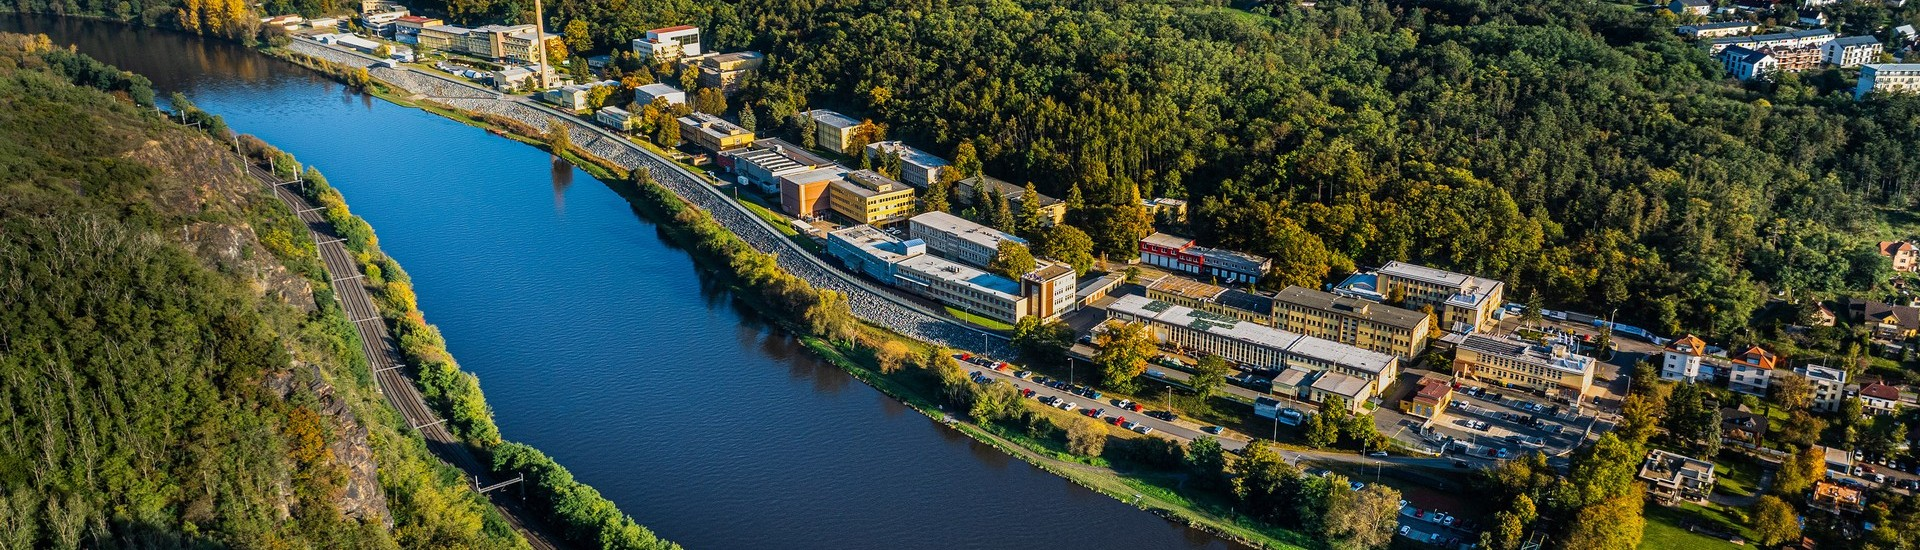
\includegraphics[height=0.38\paperheight]{figures/ujv_jaderne-udoli_dron_2024_3_4k.jpg}%
        };
      \end{scope}

      % Gradient fade from photo into NCALPrimary
      \fill[NCALPrimary, path fading=north]
        ($(current page.north west)+(0,-0.22\paperheight)$)
        rectangle
        ($(current page.north east)+(0,-0.40\paperheight)$);

      % Long NCALSecondary divider with equal page margins.
      \fill[NCALSecondary]
        ($(current page.north west)+(0.085\paperwidth,-0.555\paperheight)$)
        rectangle ++(0.83\paperwidth,0.0028\paperheight);

      % ---- Title block ----
      \node[
        anchor=north west,
        text width=0.62\paperwidth,
        align=left,
        text=NCALWhite
      ] at ($(current page.north west)+(0.085\paperwidth,-0.58\paperheight)$) {%
        {\fontsize{28}{34}\selectfont\bfseries
          NCAL Characterization\par}
        \vspace{0.42em}
        {\fontsize{18.5}{23}\selectfont\bfseries
          at \NCALInstitute\par}
        \vspace{0.55em}
        {\fontsize{14}{18}\selectfont\color{NCALSecondary}\bfseries
          Working Document\par}
        \vspace{1.7em}
        {\fontsize{12}{16}\selectfont \@author\par}
        \vspace{0.3em}
        {\fontsize{10.5}{14}\selectfont\color{NCALWhite!65!NCALPrimary}
          \NCALInstitute\par}
        \vspace{0.3em}
        {\fontsize{10.5}{14}\selectfont\color{NCALWhite!65!NCALPrimary}
          \@date\par}
      };

      % ---- NCAL detector photo – larger, right-aligned, centered on the Rez image baseline ----
      \node[anchor=east, inner sep=2.5pt,
            fill=NCALWhite,
            draw=NCALSecondary, line width=1pt]
        at ($(current page.north east)+(-0.085\paperwidth,-0.38\paperheight)$) {%
          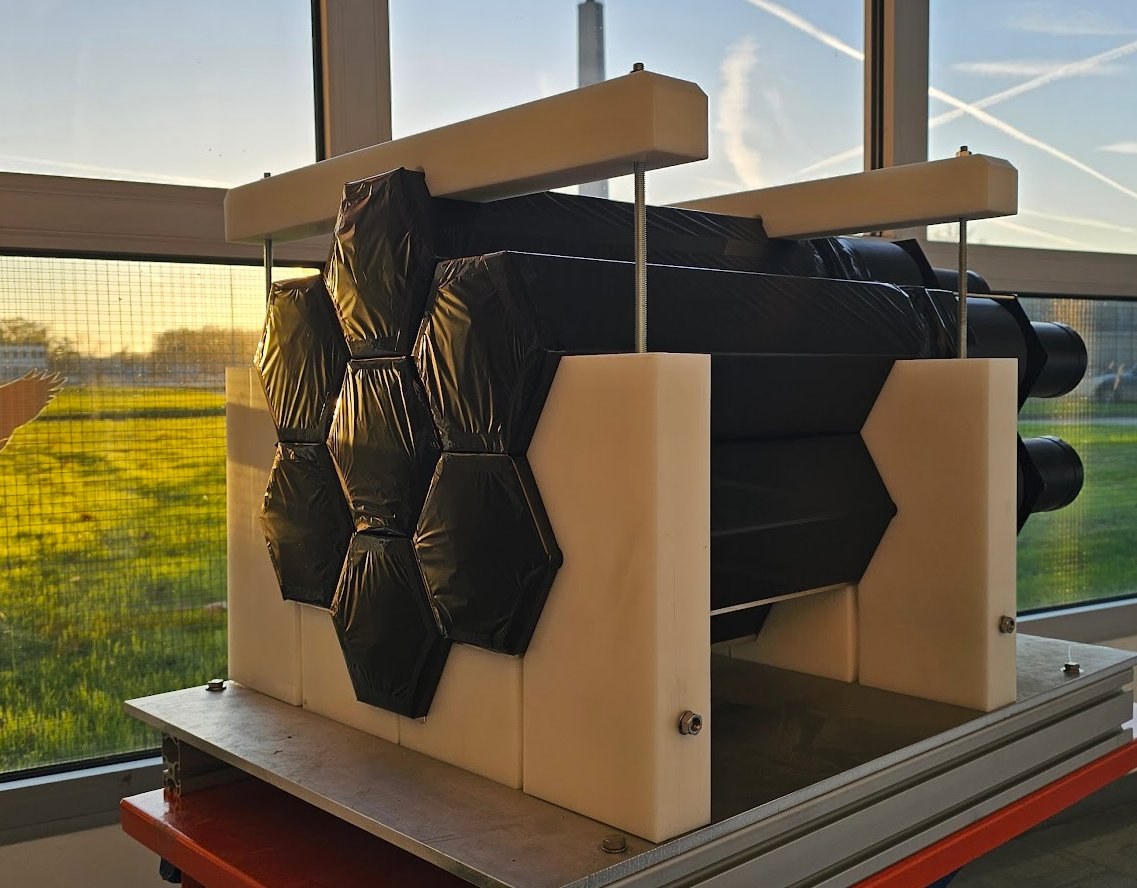
\includegraphics[width=0.24\paperwidth]{figures/NCAL.jpg}%
        };

      % ---- Bottom-right collaborator badge ----
      \fill[NCALSecondary]
        ($(current page.south east)+(-0.280\paperwidth,0.105\paperheight)$)
        rectangle ++(0.195\paperwidth,0.0015\paperheight);

      \node[anchor=south east,
            text=NCALWhite!50!NCALPrimary,
            font=\fontsize{6.8}{8}\selectfont]
        at ($(current page.south east)+(-0.085\paperwidth,0.109\paperheight)$) {%
          {\addfontfeatures{LetterSpace=4.0}COLLABORATING INSTITUTIONS}};

      \fill[NCALWhite, rounded corners=3pt]
        ($(current page.south east)+(-0.280\paperwidth,0.058\paperheight)$)
        rectangle ++(0.195\paperwidth,0.024\paperheight);

      \node[anchor=center]
        at ($(current page.south east)+(-0.1825\paperwidth,0.070\paperheight)$) {%
          
\includegraphics[width=0.182\paperwidth,trim=17 5 20 7,clip]{figures/collaborators.png}%
        };
    \end{tikzpicture}

    \null
  \end{titlepage}%
  \nopagecolor
  \restoregeometry
}
\makeatother